\documentclass[a4paper, 10pt]{article}
\usepackage[russian]{babel}
\usepackage{geometry}
\usepackage{setspace}
\usepackage[document]{ragged2e}
\usepackage[none]{hyphenat}
\usepackage{sectsty}
\usepackage{indentfirst}
\usepackage{titlesec}
\usepackage{longtable}
\usepackage{subcaption}
\usepackage{graphicx}

\babelfont{rm}{Times New Roman}

\title{ 
	\begin{flushleft}
		\begin{spacing}{1.25}
		 	\fontsize{14pt}{20pt}\selectfont УДК 004.9
		\end{spacing}
	\end{flushleft}  
	\textbf{
			\fontsize{14pt}{0pt}\selectfont	СТАНДАРТИЗАЦИЯ В СФЕРЕ ОБМЕНА ЦИФРОВЫХ ФИНАНСОВЫХ АКТИВОВ
		}
	}
\author{\textbf{Гаджиев А.М.}}
\date{}

\geometry{
	top=0.5cm,
	bottom=2cm,
	left=2cm,
	right=2cm
}

\captionsetup[longtable]{justification=raggedleft,singlelinecheck=false,skip=2pt,font={it}}
\captionsetup[figure]{belowskip=3pt, name=Рисунок, labelsep=period, belowskip=-12pt}

\graphicspath{ {./images/} }

\sectionfont{\fontsize{10}{0}\selectfont \textbf}
\titleformat{\section}{\normalfont\bfseries}{\thesection}{1em}{}
\titlespacing*{\section}{0.5cm}{13.8pt}{3pt}

\begin{document}	
	\maketitle
	\leftskip 0.5cm
	\begin{raggedleft}
	 \textit{МИРЭА - Российский технологический университет, 119454, Россия, г. Москва, проспект Вернадского, 78, e-mail: yudaarsen.ca@gmail.com
	 }
	\end{raggedleft}
	
	\justifying
	\tolerance = 9999
	\leftskip 0cm
	
	\vspace{3pt}
	\hrule height 2pt
	\vspace{3pt}
	
	\noindent \textbf{Цифровые финансовые активы являются новым финансовым инструментом в Российской Федерации. На сегодняшний день существует возможность приобретения ЦФА в момент его выпуска. Вторичный оборот ЦФА доступен только с привлечением оператора обмена. Быстрая настройка взаимодействия между оператором информационной системы и оператором обмена является важным аспектом для развития и повышения доступности инструмента. Достичь этого возможно путем стандартизации данного взаимодействия. В статье приведено сравнение цифровых финансовых активов с существующими открытыми блокчейн-платформами. Проанализированы стандарты EIP, используемые для реализации токенов на платформе Ethereum и ряде других платформ, и описана их применимость в сфере обмена цифровых финансовых активов}
	
	\vspace{3pt}
	\hrule height 2pt
	\vspace{6pt}
	
	\noindent Ключевые слова: ЦФА, цифровые финансовые активы, Ethereum, смарт-контракт, HyperLedger, EIP, блокчейн.
	
	\begin{center}
		\begin{spacing}{1.5}
			\textbf{\fontsize{14pt}{0}\selectfont STANDARDIZATION IN THE EXCHANGE OF DIGITAL FINANCIAL ASSETS}
		\end{spacing}
		\vspace{\baselineskip}
		\textbf{\fontsize{14pt}{0}\selectfont Gadzhiev A.M.}
	\end{center}
	
	\leftskip 0.5cm
	\begin{raggedleft}
		\textit{MIREA - Russian Technological University, 119454, Moscow, 78 Vernadskogo Avenue, Russia, e-mail: yudaarsen.ca@gmail.com}
	\end{raggedleft}
	
	\leftskip 0cm
	
	\vspace{3pt}
	\hrule height 2pt
	\vspace{3pt}
	
	\noindent \textbf{Digital financial assets are a new financial instrument in the Russian Federation. Today, it is possible to purchase DFA at the time of its issuance. Secondary turnover of DFA is available only with the involvement of the exchange operator. Quick interaction arrangement between the information system operator and the exchange operator is an important aspect for the development and increasing the availability of the instrument. This can be achieved by standardizing this interaction. The article compares digital financial assets to existing open blockchain platforms. The EIP standards, that are used for the implementation of tokens on the Ethereum platform and a number of other platforms, are analyzed and their applicability to the exchange of digital financial assets is described.}
	
	\vspace{3pt}
	\hrule height 2pt
	\vspace{6pt}
	
	\noindent Keywords: DFA, digital financial assets, Ethereum, smart-contract, HyperLedger, EIP, blockchain.
	
	
	\section*{Введение}
	
	Цифровые финансовые активы — это новый финансовый инструмент, набирающий все большую популярность в Российской Федерации. Применение цифровой формы финансовых активов способствует упрощению работы с ними и сокращению издержек при выпуске активов эмитентом. Выпуск, учет и обращение цифровых финансовых активов регламентируется Федеральным законом от 31.07.2020 № 259-ФЗ «О цифровых финансовых активах, цифровой валюте и о внесении изменений в отдельные законодательные акты Российской Федерации» \cite{ru:fz-259}. Цифровые финансовые активы определены законом в качестве цифровых прав, а именно:
	\begin{itemize}
		\itemsep0em
		\item[--] денежные требования к эмитенту;
		\item[--] участие в капитале непубличных акционерных обществ;
		\item[--] права по ценным бумагам.
	\end{itemize}
	
	Выпуск, учет и обращение ЦФА осуществляются в информационных системах на основе технологии распределенного реестра. Технология систем распределенного реестра представляет собой новый подход к созданию баз данных, ключевой особенностью которого является отсутствие единого центра управления \cite{ru:roadmap}. Технология широко применяется для создания криптовалют и токенов. Популярные платформы, такие как Bitcoin и Ethereum, являются открытыми сетями, участником (узлом) в которых может стать любой желающий. Для того чтобы стать узлом открытой сети достаточно установить специальное программное обеспечение, реализующее протоколы сети. В отличие от существующих платформ, реализующих технологию распределенного реестра, информационная система, в которой осуществляется выпуск, учет и обращение ЦФА, должна иметь свои правила, в том числе ограничивающие круг пользователей этой системы. Эксплуатацию информационной системы осуществляет оператор информационной системы. В таблице \ref{table:characteristics} приведен сравнительный анализ по ряду характеристик открытых блокчейн-платформ и информационных систем, в которых осуществляется выпуск ЦФА.
	
	\begin{longtable}{|p{3.5cm}|p{6.1cm}|p{6.2cm}|}
		\caption{Описание характеристик открытых блокчейн-платформ и ИС ЦФА}
		\label{table:characteristics}\\
		\hline
		
		\textbf{Характеристика} 
		& \textbf{Открытые блокчейн-платформы} 
		& \textbf{Информационные системы, в которых осуществляется выпуск ЦФА}\\
		\hline
		
		\textbf{Доступность}
		& Любой пользователь имеет возможность получить доступ к платформе
		& Доступ ограничен и регламентирован правилами информационной системы\\
		\hline
		
		\textbf{Нормативно-правовое регулирование}
		& Отсутствует
		& Деятельность регулируется нормативно-правовыми актами Российской Федерации\\
		\hline
		
		\textbf{Возможность восстановления доступа}
		& Отсутствует. При потере ключа получить доступ к криптовалюте на платформе невозможно
		& Оператор информационной системы обязан обеспечить возможность восстановления доступа\\
		\hline
		
		\textbf{Внешнее управление записями в реестре}
		& Отсутствует. Узлы взаимодействуют между собой только на основании протоколов, влияние «из вне» исключено
		& Оператор информационной системы обязан проводить изменения в распределенном реестре в соответствии с исполнительными документами\\
		\hline
		
		\textbf{Анонимность}
		& Для использования платформы не требуется указание персональных данных
		& Оператор информационной системы обязан осуществлять ведение реестра пользователей, хранить и предоставлять по запросу информацию о пользователях, содержащую персональные данные \cite{ru:cb}\\
		\hline
	\end{longtable}
	
	Открытые блокчейн-платформы реализуют возможность обмена криптовалютой (например, платформа Bitcoin), а также токенами (например, платформа Ethereum). Токены создаются на базе технологии смарт-контрактов. Смарт-контракт — это размещенный в распределенном реестре программный код, с которым можно взаимодействовать с помощью API. Тот факт, что код размещен в распределенном реестре, обеспечивает его неизменность. В технологии распределенного реестра важным аспектом является достижение консенсуса между узлами сети, таким образом, алгоритмы, заложенные в смарт-контракте, должны быть детерминированными, иначе консенсус не может быть достигнут, поскольку каждый узел будет получать новый результат выполнения кода. 
	
	Платформа Ethereum и многие другие платформы, позволяющие использовать смарт-контракты, реализуют подход, при котором новая транзакция сначала рассылается по всей сети, а затем узлы собирают транзакции в блоки, верифицируют их и выполняют код \cite{ru:eth}. В этом случае для обеспечения детерминированности алгоритма используются специальные языки программирования (например, Solidity). В существующих информационных системах, в которых осуществляется выпуск, учет и обращение ЦФА, применяется технология HyperLedger, позволяющая гибко настраивать распределенный реестр для поставленных целей \cite{ru:atomyze, ru:rules}. HyperLedger Fabric использует отличный от платформы Ethereum подход, при котором происходит в первую очередь выполнение транзакций определенным подмножеством узлов \cite{ru:hyperledger}. Такой подход позволяет использовать для написания смарт-контрактов популярные языки программирования (например, Java или Python).
	
	Цифровой финансовый актив выпускается эмитентом в соответствии с решением о выпуске ЦФА. В информационной системе, в которой выпускается ЦФА, имеется возможность проводить сделки, связанные с приобретением ЦФА пользователями платформы. Для осуществления вторичного оборота, то есть для проведения сделок купли-продажи или обмена ЦФА между владельцами, требуется участие оператора обмена цифровых финансовых активов (рисунок  \ref{figure:schema}). 
	
	Оператор обмена ЦФА – это организация, обеспечивающая заключение сделок с ЦФА путем сбора и сопоставления разнонаправленных заявок на совершение таких сделок либо путем участия за свой счет в сделке с цифровыми финансовыми активами в качестве стороны такой сделки в интересах третьих лиц \cite{ru:fz-259}. Оператору обмена необходимо настраивать взаимодействие с каждой конкретной информационной системой для выполнения своих функций. Повышение эффективности работы оператора, а также сокращение времени для интеграции с новой информационной системой может быть достигнуто путем разработки и реализации стандартов. 
	
	\begin{figure}
		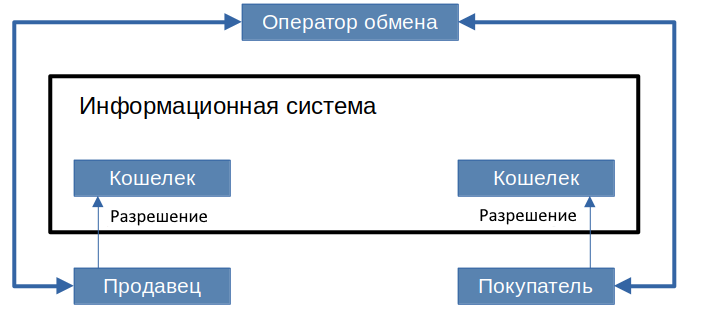
\includegraphics[width=16cm]{schema}
		\centering
		\caption{Схема обмена цифровых финансовых активов}
		\label{figure:schema}
	\end{figure}
	
	\section*{Анализ стандартов платформы Ethereum}
	
	В настоящее время существуют биржи, осуществляющие свою деятельность в открытых блокчейн-платформах. С появлением платформы Ethereum создается множество различных токенов, которые покупаются, продаются и обмениваются на биржах. Поскольку для создания токена в открытой блокчейн-платформе достаточно развертывания смарт-контракта, были разработаны правила, обеспечивающие возможность биржам работать с новыми токенами средствами стандартизованных интерфейсов. Учитывая разницу по ряду характеристик между отрытыми блокчейн-платформами и информационными системами ЦФА, а также тот факт, что смарт-контракты в ИС ЦФА разрабатываются на популярных языках программирования, существующие стандарты не подходят для применения в сфере обмена ЦФА, но подходы, описанные в них, могут быть использованы при разработке новых стандартов. 
	
	Стандартны платформы Ethereum называются Ethereum Improvement Proposals (EIP). Существуют следующие типы EIP \cite{ru:eip}:
	
	\begin{enumerate}
		\itemsep0em
		\item Standard Track. Описывает существенные изменения реализации платформы (например, изменения протокола).
		\item Core. Улучшения, требующие ответвления консенсуса.
		\item Networking. Касаются протоколов сетевого взаимодействия в рамках сети.
		\item Interface. Улучшения спецификаций и стандартов клиентского API.
		\item ERC. Стандарты на уровне приложений, включая стандарты смарт-контрактов.
		\item Meta. Описывает процесс, связанный с Ethereum, или предлагает изменение в процессе.
		\item Informational. Описывает общие рекомендации, но не предлагает новую функцию.
	\end{enumerate}
	
	В настоящее время в Российской Федерации в качестве цифровых финансовых активов эмитируются, в основном, денежные требования к эмитенту с фиксированной суммой, либо привязанные к курсу драгоценного металла \cite{ru:dfa, ru:lighthouse}. Каждое такое денежное требование можно интерпретировать в качестве токена, поэтому для анализа подходов, описанных в EIP, следует рассмотреть тип ERC. 
	
	EIP типа ERC описывают два основных вида токенов: взаимозаменяемый и не взаимозаменяемый. Их отличие заключается в том, что при обмене взаимозаменяемого токена пользователь получит ту же ценность, которую имел, а при обмене не взаимозаменяемого токена, пользователь получит новую ценность. В качестве примера взаимозаменяемого токена можно привести монеты одного номинала или единицу игровой валюты, а не взаимозаменяемым токеном является, например, оцифрованное произведение искусства. В таблице \ref{table:eip} приводятся EIP, описывающие интерфейс токенов разного вида.
	
	\begin{longtable}{|p{3.5cm}|p{6.1cm}|p{6.2cm}|}
		\caption{EIP, описывающие интерфейс токенов}
		\label{table:eip}\\
		\hline
		
		\textbf{Вид токена} 
		& \textbf{EIP} 
		& \textbf{Описание}\\
		\hline
		
		Взаимозаменяемый
		& EIP-20: Token Standard
		& Описывает интерфейс взаимозаменяемого токена\\
		\hline
		
		Не взаимозаменяемый
		& EIP-721: Non-Fungible Token Standard
		& Описывает интерфейс не взаимозаменяемого токена\\
		\hline
		
		Взаимозаменяемый
		& EIP-777: Token Standard
		& Улучшение стандарта EIP-20\\
		\hline
		
		Взаимозаменяемый и не взаимозаменяемый
		& EIP-1155: Multi Token Standard
		& Интерфейс смарт-контракта, который может иметь как взаимозаменяемые токены, так и не взаимозаменяемые\\
		\hline
		
		Не взаимозаменяемый
		& EIP-3525: Semi-Fungible Token
		& Содержит понятие количества к токену стандарта EIP-721, которое можно обменивать\\
		\hline
	\end{longtable}
	
	Поскольку денежное требование эмитируется с одинаковым условием погашения, то при обмене такого денежного требования на денежное требование того же типа, пользователь получит ту же ценность. Таким образом, ЦФА, являющиеся цифровыми правами, удостоверяющими денежные требования к эмитенту определенной суммы, то есть без накопления процентов по конкретному ЦФА, могут рассматриваться в качестве взаимозаменяемых токенов.
	Рассмотрим основные функции интерфейса, описанного в стандарте EIP-20, и их применимость к обмену ЦФА (таблица \ref{table:erc20}).
	
	Стандарт EIP-777 вводит термин «Оператор», который используется в ситуациях перевода токенов третьим лицом на основании разрешения. Пользователь может предоставить доступ нескольким операторам одновременно. Также стандарт предусматривает наличие оператора по умолчанию, что является необходимым в сфере обмена ЦФА, чтобы оператор информационной системы мог выполнять требования законодательства (например, перевод ЦФА по исполнительным документам). Добавляются новые функции authorizeOperator и revokeOperator, обеспечивающие управление разрешением для конкретного оператора. Стандартом также добавляется понятие детализации (функция granularity), подразумевающее минимальное количество токенов, с которыми можно осуществить какую-либо операцию. Такой подход применим для ЦФА, имеющих ограничение на минимальное количество токенов, доступных для покупки в рамках одного лота. 
	
	\begin{longtable}{|p{3.5cm}|p{6.1cm}|p{6.2cm}|}
		\caption{Основные функции интерфейса EIP-20}
		\label{table:erc20}\\
		\hline
		
		\textbf{Наименование функции} 
		& \textbf{Описание} 
		& \textbf{Применимость к обмену ЦФА}\\
		\hline
		
		transfer
		& Перевести токены по адресу
		& Не может быть использовано, поскольку вторичный оборот ЦФА осуществляется при посредничестве оператора обмена ЦФА, а не самим владельцем в ИС\\
		\hline
		
		approve
		& Разрешить определенному адресу переводить токены до определенного лимита
		& Функция применима в случае автоматизации предоставления разрешения оператору пользователем платформы\\
		\hline
		
		transferFrom
		& Перевод токенов с кошелька третьим лицом на основании разрешения
		& Необходимая функция для возможности оператора обмена выполнять свои функции, а также для оператора информационной системы для выполнения требований, предусмотренных законодательством\\
		\hline
	\end{longtable}
	
	\section*{Заключение}
	
	Механизм обмена цифровых финансовых активов схож с работой бирж, которые работают на открытых блокчейн-платформах. Подходы, описанные в стандартах, которые были сформированы с появлением и развитием платформ, реализующих технологию смарт-контрактов, могут являться основой для разработки новых стандартов в сфере обмена ЦФА. В рассмотренных стандартах заложен механизм осуществления операций с токенами третьими лицами. Такой подход является необходимым с точки зрения выполнения требований законодательства оператором информационной системы и для осуществления основных функций оператором обмена. Адаптация данного подхода и его применение в информационных системах ЦФА позволит упростить настройку взаимодействия операторов обмена с платформами и способствует дальнейшему развитию ЦФА в Российской Федерации в качестве нового и доступного финансового инструмента.
	\newline
	
	\makeatletter
\renewcommand\@biblabel[1]{#1.}
\makeatother

Список литературы
\hrule height 2pt

\renewcommand{\refname}{}
\vspace{-\baselineskip}
\begin{thebibliography}{10}
	\bibitem{ru:fz-259} Федеральный закон от 31.07.2020 № 259-ФЗ «О цифровых финансовых активах, цифровой валюте и о внесении изменений в отдельные законодательные акты Российской Федерации» (Дата обращения 10.01.2023)
	\bibitem{ru:roadmap} Министерство цифрового развития, связи и массовых коммуникаций Российской Федерации. Дорожная карта развития «сквозной» цифровой технологии «Системы распределенного реестра». Режим доступа: https://digital.gov.ru/ru/documents/6670/ (Дата обращения 10.01.2023)
	\bibitem{ru:cb} Указание Банка России от 19.11.2020 N 5625-У «О документах, предусмотренных частью 4 статьи 8 Федерального закона от 31 июля 2020 года N 259-ФЗ «О цифровых финансовых активах, цифровой валюте и о внесении изменений в отдельные законодательные акты Российской Федерации», и требованиях к их хранению». Режим доступа: https://www.cbr.ru/Queries/UniDbQuery/File/90134/1190 (Дата обращения 10.01.2023)
	\bibitem{ru:dfa} Цифровые финансовые активы – СберБанк. Решение о выпуске цифровых финансовых активов. ПАО «Сбербанк России». Режим доступа: http://www.sberbank.ru/common/img/uploaded/legal/docs/digital-assets/ reshenie-o-vypuske-09122022.pdf (Дата обращения 10.01.2023)
	\bibitem{ru:lighthouse} Лайтхаус – цифровая финансовая экосистема. Решение №2 о выпуске цифровых финансовых активов (токенов) с оплатой денежными средствами от «20» октября 2022 г. Режим доступа: https://www.cfa.digital/disclosure (Дата обращения 11.01.2023)
	\bibitem{ru:eth} Ethereum. Mining. Режим доступа: https://ethereum.org/en/developers/docs/consensus-mechanisms/pow/mining/ (Дата обращения 11.01.2023)
	\bibitem{ru:atomyze} Atomyze. Режим доступа: https://atomyze.ru/press-reliz (Дата обращения 11.01.2023)
	\bibitem{ru:rules} Правила информационной системы Сбера, в которой осуществляется выпуск цифровых финансовых активов. Режим доступа: http://www.sberbank.ru/common/img/uploaded/legal/docs/digital-assets/pravila\_inf\_sistemy.pdf (Дата обращения 11.01.2023)
	\bibitem{ru:hyperledger} HyperLedger Fabric. Docs. Режим доступа: https://hyperledger-fabric.readthedocs.io/en/release-2.5/whatis.html (Дата обращения 11.01.2023)
	\bibitem{ru:eip} Ethereum Improvement Proposals. Режим доступа: https://eips.ethereum.org/ (Дата обращения 11.01.2023)
\end{thebibliography}

\vspace{\baselineskip}

References
\vspace{3pt}
\hrule height 2pt
\renewcommand{\refname}{}
\vspace{-\baselineskip}
\begin{thebibliography}{10}
	\bibitem{en:fz-259} The federal law of the Russian Federation of 31.07.2020 № 259-FZ «On digital financial assets, digital currency and on amendments to certain legislative acts of the Russian Federation» (Accessed 10.01.2023)
	\bibitem{en:roadmap} Ministry of Digital Development, Communications and Mass Media of the Russian Federation. Roadmap for the development of "end-to-end" digital technology "Distributed Registry System". Access mode: https://digital.gov.ru/ru/documents/6670/ (Accessed 10.01.2023)
	\bibitem{en:cb} Bank of Russia Directive of 19.11.2020 N 5625-U «On the documents stipulated in part 4 of Article 8 of the Federal Law of July 31, 2020 N 259-FZ "On Digital Financial Assets, Digital Currency and on Amendments to Certain Legislative Acts of the Russian Federation", and requirements for their storage». Access mode: https://www.cbr.ru/Queries/UniDbQuery/File/90134/1190 (Accessed 10.01.2023)
	\bibitem{en:dfa} Digital financial assets – SberBank. The decision to issue digital financial assets. Sberbank of Russia. Access mode: http://www.sberbank.ru/common/img/uploaded/legal/docs/digital-assets/reshenie-o-vypuske-09122022.pdf (Accessed 10.01.2023)
	\bibitem{en:lighthouse} Lighthouse – digital financial ecosystem. Decision No. 2 on the issue of digital financial assets (tokens) with payment in cash dated «20» October 2022. Access mode: https://www.cfa.digital/disclosure (Accessed 11.01.2023)
	\bibitem{en:eth} Ethereum. Mining. Access mode: https://ethereum.org/en/developers/docs/consensus-mechanisms/pow/mining/ (Accessed 11.01.2023)
	\bibitem{en:atomyze} Atomyze. Access mode: https://atomyze.ru/press-reliz (Accessed 11.01.2023)
	\bibitem{en:rules} Rules of the information system of Sbera, in which digital financial assets are issued. Access mode: http://www.sberbank.ru/common/img/uploaded/legal/docs/digital-assets/pravila\_inf\_sistemy.pdf (Accesed 11.01.2023)
	\bibitem{en:hyperledger} HyperLedger Fabric. Docs. Access mode: https://hyperledger-fabric.readthedocs.io/en/release-2.5/whatis.html (Accessed 11.01.2023)
	\bibitem{en:eip} Ethereum Improvement Proposals. Access mode: https://eips.ethereum.org/ (Accessed 11.01.2023)
\end{thebibliography}
	
\end{document}